\lhead{\emph{Design}}
\chapter{Design}
This chapter first explains the design methods used and the most important design activities and choices made in the design process. Based on this process the final prototype design is presented at the end of the chapter.

\section{Design model and methods}
In this section the model used for designing the final prototype is presented including the different techniques used throughout the design process.

The related works conducts the foundations for an early first prototype. This prototype will then go through an iterative design process, taking a user centered approach. This will enable specifications to emerge during the process and these learnings and modifications will result in new experiments and prototypes. This iterative design model is illustrated in figure \ref{fig:iterative}.

\begin{figure}[htbp]
	\centering
		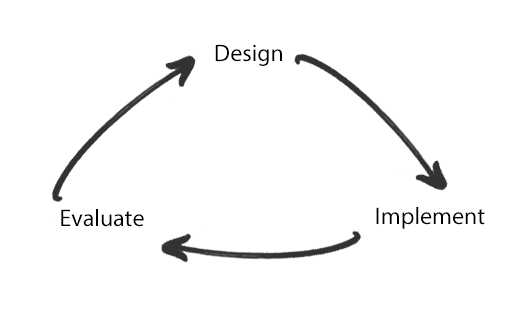
\includegraphics[width=0.6\textwidth,height=\textheight,keepaspectratio]{./Figures/iterative.png}
		\rule{35em}{0.5pt}
	\caption[Iterative Design Model]{Iterative Design Model}
	\label{fig:iterative}
\end{figure}

\subsection{Envisionment}
One of the goals with the final system is that it should be eyes-free i.e. the user should not depend on a visual screen UI at the end. Despite this goal, the use of a screen to visualize e.g. a virtual menu, can be helpful in the design process. This will enable test users to get a quicker and better understanding of how the interaction works. In this design process a mobile device screen will be used for envisionment - this is also called a hifi prototype or software prototype \cite{benyon_designing_2010}.

More concretely audio sources and the users head position including rotation will be mapped visually to a screen dynamically during user interaction. An example of this screen is shown in figure ?

\section{Design process}
This section starts out by describing the first experimental prototype design inspired from previous research work and then each iteration including user feedback and design changes and experiments. More specifically the design completed 2 iterations before the final prototype design.

\subsection{Initial prototype design considerations}
Before we started to reason about initial design choices we started out by defining what the system actually needed in order to evaluate and revise the hypothesis from the problem statement.

% intro, track exploring
First of all we wanted the system to be able to play music. This is in itself a trivial task but as we the same time wanted to control the system only with with head gestures and audio output a traditional music player includes too many options e.g. play, pause, stop, next/previous, volume, equalizer, track exploring, etc for the scope of this thesis. All the alternative music players mentioned in chapter \ref{sec:relatedwork} is limited to simple commands like play, stop, next/previous and volume. Taking it a step further we wanted to evaluate the track exploring part i.e. navigating to a preferred track and playing it. This made et clear that some kind of auditory menu with tracks as menu items was needed and although not music players the related systems from chapter \ref{sec:relatedwork} using auditory menus could inspire to an intital menu design.

% Auditory menu, exocentric, head rotation constraints
When looking at the different related auditory menu designs we needed to find a design that fitted into the context of the user activity i.e. biking and also user interaction modality. E.g. in a biking scenario the user should have eyes on the road thereby constraining the head rotation. Park et. al \cite{park_gaze-directed_2011} showed good results with a 2D grid menu. It should be taken into account that their audio output consists of simple speech commands e.g. speech recorded numbers. We want to present multiple music streams (non-speech audio) and studies have shown that when presenting multiple non-speech audio streams simultanously in a spatial audio space, segregating the audio streams horizontically has a better effect than vertical alignment [TODO: ref]. It seemed that a circular auditory menu could be a good starting point and both Kajastila and Lokki \cite{kajastila_interaction_2013} and also Brewster et. al \cite{brewster_multimodaleyes-freeinteraction_2003} evaluated this kind of menu design with good results.

[TODO: Image/prototype sketch?]

\begin{figure}[htbp]
	\centering
		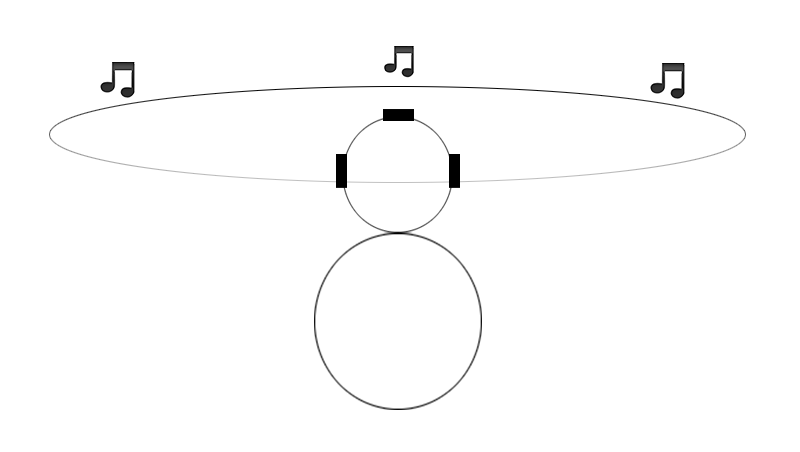
\includegraphics[width=0.6\textwidth,height=\textheight,keepaspectratio]{./Figures/sounddesign.png}
		\rule{35em}{0.5pt}
	\caption[Soundscape Design]{Soundscape Design - Visualising how the circular auditory menu surrounds a person (viewed from the persons back)}
	\label{fig:sounddesign}
\end{figure}

% Circular menu design, head gestures
While placing music streams in a circular way around a users audio space we needed a way of navigating to and chosing a specific track. The Brewster et. al \cite{brewster_multimodaleyes-freeinteraction_2003} system uses directed nods to choose an item but this limits the number of items to 4 (1 for every 90 degrees) as a nod in 45 degrees

The inititial interaction design was inspired from Kajastila and Lokkis system although they used hand gestures as modality input. 

For navigating and choosing menu items

[TODO: egocentric vs exocentric audio output, Brewster system good ref \cite{vazquez-alvarez_eyes-free_2011}]

% Summarising

[TODO]
In this project multiple audio sources (music tracks) are presented for the user at the same time but none of them requires a respond i.e. the focus is on selective-attention tasks.

\subsection{Fixed head position experiment}

\subsection{Dynamic head position experiment}

\subsection{Head gestures}

Recording user gestures

Navigating the menu

Adjusting sensor data input - accelerometer problem when biking


\section{Final prototype design}

% \subsection{Audio menu structure}

%Several studies show that circular auditory menus are the way to go because of horizontally positioned sounds , HRTF, 3D audio...

%Human head normally can be rotated about 140 degrees for shaking and 100 degrees for nodding \cite{lopresti_neck_2000}.

%\subsection{Navigation controls}

% prototyping, iterative design process

TODO: New suggestion for sections

Design space
- Requirements
- Pros/cons with different design choices

Soundscape design
- Music
- Horizontal argument
- Simultanous sounds, exploring, cocktail party effect argument
- Experimental design, sounds perceived, zoom effect, user should detect sound direction (which track)

Menu
- Navigation
- Head gestures
- Activating menu
- Figure showing levels of menu
- Feedback when gesture recognized






% OLD STUFF
%An experimental prototype should be developed and tested. 3 types of menus where a test user should perform head gesture interaction to solve small tasks. User is observed and feedback should be given.

%A final prototype should be designed with knowledge from the experimental evaluation. This prototype will go through a "real life" evaluation. It will be evaluated through several days where the user will use the new head gesture based music application and the traditional music application while biking. Again small task could be performed and it could be tested through the users normal use of his/her music application, ending up in a comparison of the traditional vs the new interaction system.


